%  article.tex (Version 3.3, released 19 January 2008)
%  Article to demonstrate format for SPIE Proceedings
%  Special instructions are included in this file after the
%  symbol %>>>>
%  Numerous commands are commented out, but included to show how
%  to effect various options, e.g., to print page numbers, etc.
%  This LaTeX source file is composed for LaTeX2e.

%  The following commands have been added in the SPIE class 
%  file (spie.cls) and will not be understood in other classes:
%  \supit{}, \authorinfo{}, \skiplinehalf, \keywords{}
%  The bibliography style file is called spiebib.bst, 
%  which replaces the standard style unstr.bst.  

%%\documentclass[]{spie}  %>>> use for US letter paper
\documentclass[a4paper]{spie}  %>>> use this instead for A4 paper
%%\documentclass[nocompress]{spie}  %>>> to avoid compression of citations
%% \addtolength{\voffset}{9mm}   %>>> moves text field down
%% \renewcommand{\baselinestretch}{1.65}   %>>> 1.65 for double spacing, 1.25 for 1.5 spacing 
%  The following command loads a graphics package to include images 
%  in the document. It may be necessary to specify a DVI driver option,
%  e.g., [dvips], but that may be inappropriate for some LaTeX 
%  installations. 
\usepackage[]{graphicx}
\usepackage{amsmath}
\usepackage{multirow}
\usepackage{url}

\title{Predicting Chroma from Luma with Frequency Domain Intra Prediction}

%>>>> The author is responsible for formatting the 
%  author list and their institutions.  Use  \skiplinehalf 
%  to separate author list from addresses and between each address.
%  The correspondence between each author and his/her address
%  can be indicated with a superscript in italics, 
%  which is easily obtained with \supit{}.

\author{Nathan E. Egge
\skiplinehalf
Mozilla, Mountain View, USA
}

%>>>> Further information about the authors, other than their 
%  institution and addresses, should be included as a footnote, 
%  which is facilitated by the \authorinfo{} command.

%\authorinfo{Further author information: (Send correspondence to A.A.A.)\\A.A.A.: E-mail: aaa@tbk2.edu, Telephone: 1 505 123 1234\\  B.B.A.: E-mail: bba@cmp.com, Telephone: +33 (0)1 98 76 54 32}
%%>>>> when using amstex, you need to use @@ instead of @
 

%%%%%%%%%%%%%%%%%%%%%%%%%%%%%%%%%%%%%%%%%%%%%%%%%%%%%%%%%%%%% 
%>>>> uncomment following for page numbers
% \pagestyle{plain}    
%>>>> uncomment following to start page numbering at 301 
%\setcounter{page}{301} 
 
  \begin{document} 
  \maketitle 

%%%%%%%%%%%%%%%%%%%%%%%%%%%%%%%%%%%%%%%%%%%%%%%%%%%%%%%%%%%%% 
\begin{abstract}
This paper describes a technique for performing intra prediction of the chroma
 planes based on the reconstructed luma plane in the frequency domain.
This prediction exploits the fact that while RGB to YUV color conversion has
 the property that it decorrelates the color planes globally across an image,
 there is still some correllation locally at the block level\cite{LeeCho09}.
Previous proposals compute a linear model of the spatial relationship between
 the luma plane (Y) and the two chroma planes (U and V)\cite{JCTVCB021}.
In codecs that use lapped transforms this is not possible since transform
 support extends across the block boundaries\cite{Tran2003}.
We design a frequency domain intra predictor for chroma that exploits the same
 local correlation with lower complexity than the spatial predictor and which
 works with lapped transforms.


%(need to talk about improvements over other forms of intra prediction)
%(what about complexity, fewer multiplies when predicting the model)
\end{abstract}

%>>>> Include a list of keywords after the abstract 

%\keywords{Manuscript format, template, SPIE Proceedings, LaTeX}
\keywords{Intra Prediction, Lapped Transforms, Color Image Coding, Chroma
 Correlation, Regression}

%%%%%%%%%%%%%%%%%%%%%%%%%%%%%%%%%%%%%%%%%%%%%%%%%%%%%%%%%%%%%
\section{INTRODUCTION}
\label{sec:intro}  % \label{} allows reference to this section

Still image and video codecs typically consider the problem of intra-prediction
 in the spatial domain.
A predicted image is generated on a block-by-block basis using the previously
 reconstructed neighboring blocks for reference, and the residual is encoded
 using standard entropy coding techniques.
Modern codecs use the boundary pixels of the neighboring blocks along with a
 directional mode to predict the pixel values across the target block (e.g.,
 AVC, HEVC, VP8, WebP, etc.).
These directional predictors are cheap to compute (often directly copying pixel
 values or applying a simple linear kernel), exploit local coherency (with low
 error near the neighbors) and predict hard to code features (extending sharp
 directional edges across the block).

In codecs that use lapped transforms these techniques are not applicable (e.g.,
 VC-1, JPEG-XR, Daala, etc.).
The challenge here is that the neighboring spatial image data is not available
 until {\em after} the target block has been decoded and the appropriate
 unlapping filter has been applied across the block boundaries.
Figure \ref{fig:decode} shows the decode pipeline of a codec using lapped
 transforms with a single block size.
The support used in spatial intra prediction is exactly the region that has not
 had the unlapping post-filter applied.
Note that the pre-filter has the effect of decorrelating the image along block
 boundaries so that the neighboring pixel values before unlapping are
 particularly unsuitable for use in prediction.

\begin{figure}
\begin{center}
\begin{tabular}{c}
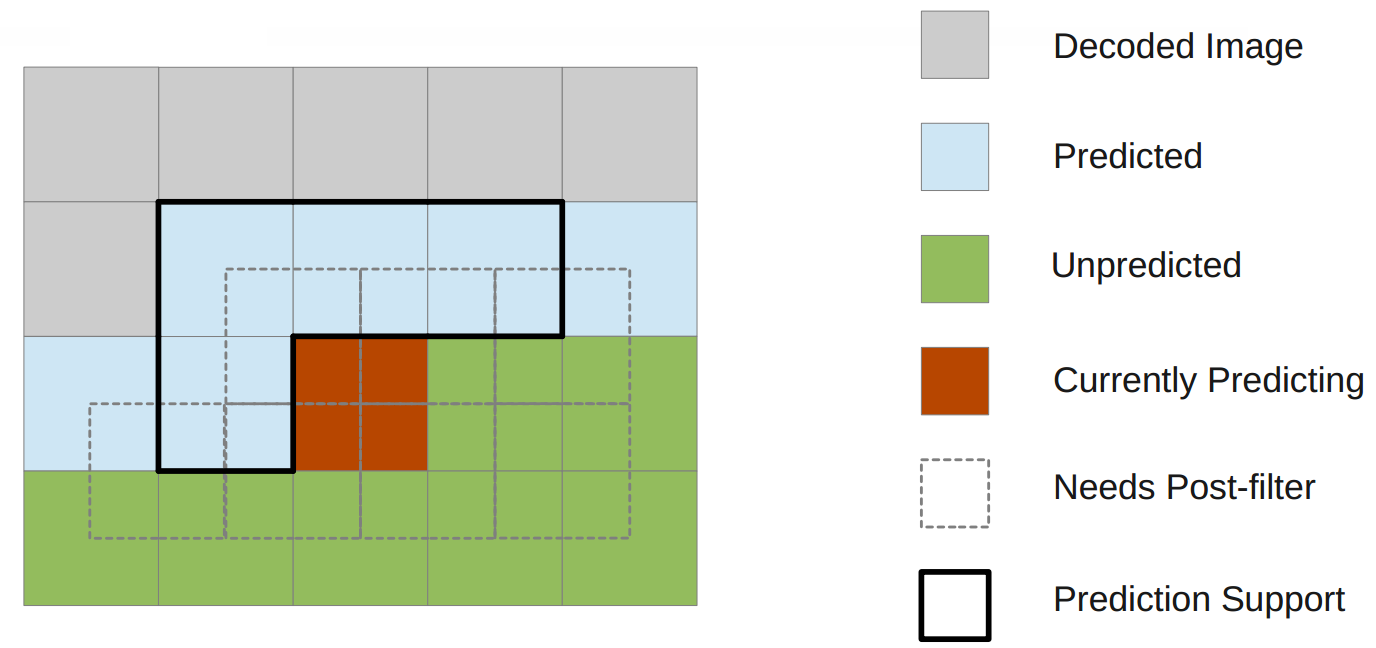
\includegraphics[natwidth=1376,natheight=646,width=4in]{daala_decode.png}
\end{tabular}
\end{center}
\caption[example]{\label{fig:decode} State of blocks in the decode pipeline of
 a codec using lapped transforms. Immediate neighbors of the target block
 (bold lines) cannot be used for spatial prediction as they still require
 post-filtering (dotted lines).}
\end{figure}

%\section{RELATED WORK}

Work has been done to use intra prediction with lapped transforms.
Modifying AVC, de Oliveira and Pesquet showed that it was possible to use the
 boundary pixels just outside the lapped region to use 4 of the 8 directional
 intra prediction modes with lapped transforms\cite{oliv2011}.
The work of Xu, Wu and Zhang considers prediction as a transform and describes
 a frequency domain intra prediction using non-overlapped blocks\cite{xuwu2009}.
The experimental Daala video codec extends this idea using machine learning to
 train sparse intra predictors\cite{DaalaDemo2}.
However this technique is computationally expensive (4 multiplies per
 coefficient) and not easily vectorized.

A promising technique was proposed by Lee and Cho to predict the chroma
 channels using the spatially coincident reconstruted luma
 channel\cite{LeeCho09}.
This was formally proposed for use in HEVC by Chen et al\cite{JCTVCB021}
 however was ultimately not selected due to the increased encoder and decoder
 running time of 20-30\%.
We propose a similar technique that adapts the spatial chroma-from-luma
 intra prediction for use with frequency-domain coefficients.
We call this algorithm frequency-domain chroma-from-luma (FD-CfL).

\section{CHROMA FROM LUMA PREDICTION}
\label{sec:chroma}

In spatial-domain chroma-from-luma, the key observation is that the local
 correlation between luminance and chrominance can be exploited using a linear
 prediction model.
For the target block, we have that the chroma values can be estimated from the
 reconstructed luma values as:
$$C(u,v) = \alpha\cdot L(u,v) + \beta$$
where the model parameters $\alpha$ and $\beta$ are computed as a linear
 least-squares regression using pairs of spatially coincident luma and chroma
 pixel values along the boundary:
\begin{align}
\alpha & = \frac{I\cdot\displaystyle\sum_i^I L_i\cdot C_i - \displaystyle\sum_i^I L_i\displaystyle\sum_i^I C_i}{I\cdot\displaystyle\sum_i^I L_i\cdot L_i - \left(\displaystyle\sum_i^I C_i\right)^2}, & \beta & = \frac{\displaystyle\sum_i^I C_i -\alpha\cdot\displaystyle\sum_i^I L_i}{I}.
\label{eqn:fit}
\end{align}

When $\alpha$ and $\beta$ are sent explicitly in the bitstream, the pairs
 $(L_i,C_i)$ are taken from the original, unmodified image.
However, the decoder can compute the same linear regression using the
 reconstructed luma and chroma planes and thus $\alpha$ and $\beta$ can be
 derived {\em implicitly} from the bitstream.
Additional computation is necessary when the choma plane is subsampled (e.g.,
 4:2:0 and 4:2:2 image data) as the luma pixel values are no longer coincident
 and must be resampled.
In the next section we show how this issue does not exist when the algorithm
 is adapted to the frequency-domain.

\section{PROPOSED ALGORITHM}
\label{sec:alg}

In codecs that use lapped transforms, the reconstructed pixel data is not
 available.
However we observe that the transform coefficients in the lapped frequency
 domain are the product of two linear transforms: the linear pre-filter
 followed by the linear forward DCT.
Thus the same assumption of a linear correlation between luma and chroma
 coefficients holds.
In addition, we can take advantage of the fact that we are in the frequency
 domain to use only a small subset of coefficients when computing our model.

The chroma values can then be estimated using frequency-domain chroma-from-luma
 (FD-CfL):
\begin{align*}
C_{DC} &= \alpha_{DC}\cdot L_{DC} + \beta_{DC} \\
C_{AC}(u,v) &= \alpha_{AC}\cdot L_{AC}(u,v)
\end{align*}
where the $\alpha_{DC}$ and $\beta_{DC}$ are computed using the linear
 regression in (\ref{eqn:fit}) with the DC coefficients of the three
 neighboring blocks: U, L and UL.
When estimating $C_{AC}(u,v)$ we can omit the constant offset $\beta_{AC}$
 as we expect the AC coefficients to be zero mean.
Additionally, we do not include all of the AC coefficients from the same three
 neighboring blocks when computing $\alpha_{AC}$.

\begin{figure}
\begin{center}
\begin{tabular}{c c c}
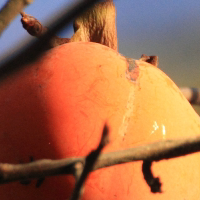
\includegraphics[natwidth=200,natheight=200,width=1.75in]{fruits-orig.png}
&
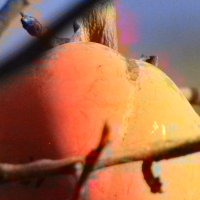
\includegraphics[natwidth=200,natheight=200,width=1.75in]{fruits-intra.png}
&
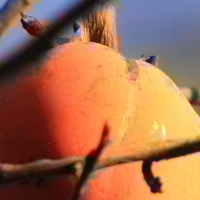
\includegraphics[natwidth=200,natheight=200,width=1.75in]{fruits-cfl.png}
\\
(a) & (b) & (c)
\end{tabular}
\end{center}
\caption[example]{\label{fig:comp} Comparison of (a) the original uncompressed
 image with composite images of (b) reconstructed luma and predicted chroma
 using Daala intra modes and (c) reconstructed luma and predicted chroma using
 FD-CfL.}
\end{figure}

It is sufficient to use the three lowest AC coefficients from the neighboring
 blocks.
This means that the number of input pairs $I$ is constant regardless of the
 size of chroma block being predicted.
Moreover, the input AC coefficients have semantic meaning: we use the
 strongest horizontal, vertical and diagonal components.
This has the effect of preserving features across the block as edges are
 correlated between luma and chroma, see the fruit and branch edges in
 Figure \ref{fig:comp}c.

\subsection{TIME-FREQUENCY RESOLUTION SWITCHING}

When image data is 4:4:4 or 4:2:0, the chroma and luma blocks are aligned so
 that the lowest 3 AC coefficients describe the same frequency range.
In codecs that support lapped transforms and multiple block sizes (or that
 support 4:2:2 image data) it is the case that the luma blocks and the chroma
 blocks are not aligned.
For example, in the Daala video codec which uses lapped transforms, the
 smallest DCT supported is 4x4.
In 4:2:0, when an 8x8 block of luma image data is split into four 4x4 blocks,
 the corresponding 4x4 chroma image data is coded as a single 4x4 block.

This is a problem for FD-CfL as it requires the reconstructed luma frequency
 domain coefficients to cover the same spatial extent.
In Daala this is overcome by borrowing a technique from the Opus audio
 codec\cite{valin2013high}.
Using Time-Frequency resolution switching (TF) it is possible to trade off
 resolution in the spatial domain for resolution in the frequency domain.
Here the four 4x4 luma blocks are {\em merged} into a single 8x8 block with
 half the time resolution and twice the frequecy resolution.
The low frequency (LF) coefficients are then used with FD-CfL, see
 Figure \ref{fig:tf}.

\begin{figure}[h]
\begin{center}
\begin{tabular}{c}
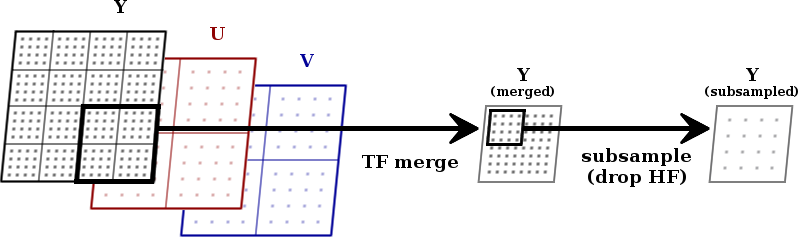
\includegraphics[natwidth=799,natheight=237,width=4in]{CfL-TF.png}
\end{tabular}
\end{center}
\caption[example]{\label{fig:tf} Using TF-merge to convert four 4x4 frequency
 domain luma blocks (Y) into a single 8x8 frequency domain block for use with
 TD-CfL when image data is 4:2:0.  Note that only the lower frequency (LF)
 portion is actually necessary and thus only that portion of the TF-merge need
 be computed.}
\end{figure}

\section{COMPLEXITY COMPARISON}

\begin{table}
\begin{center}
\begin{tabular}{|c|c|c|c|c|}
\hline
\multirow{2}{*}{Block Size} & \multicolumn{2}{|c|}{Spatial Domain} & \multicolumn{2}{|c|}{Freq. Domain} \\
\cline{2-5}
 & Mults & Adds & Mults & Adds \\
\hline
$N\times N$ & $4*N+2$ & $8*N+3$ & $2*12+2$ & $4*12+3$ \\
\hline
$4\times 4$ & 18 & 35 & 26 & 51 \\
\hline
$8\times 8$ & 34 & 67 & 26 & 51 \\
\hline
$16\times 16$\footnotemark[1] & 66 & 131 & 26 & 51 \\
\hline
\end{tabular}
\end{center}
\caption[example]{\label{tbl:comp} Comparison of (a) the original uncompressed
 image with composite images of (b) reconstructed luma and predicted chroma}
\end{table}
\footnotetext[1]{Daala does not currently handle $32\times 32$ luma blocks but will likely add support in the future.}

\section{IMPLEMENTATION}

This work is part of the Daala project\cite{DaalaWebsite}.
The full source code, including all of the FD-CfL work described in this paper
 is available in the project git repository\cite{DaalaGit}.

%%%%%%%%%%%%%%%%%%%%%%%%%%%%%%%%%%%%%%%%%%%%%%%%%%%%%%%%%%%%%
%\acknowledgments     %>>>> equivalent to \section*{ACKNOWLEDGMENTS}       
%This unnumbered section is used to identify those who have aided the authors in understanding or accomplishing the work presented and to acknowledge sources of funding.  

%%%%%%%%%%%%%%%%%%%%%%%%%%%%%%%%%%%%%%%%%%%%%%%%%%%%%%%%%%%%%
%%%%% References %%%%%

\bibliography{spie_cfl}   %>>>> bibliography data in report.bib
\bibliographystyle{spiebib}   %>>>> makes bibtex use spiebib.bst

\end{document} 
